\documentclass[journal,conference]{IEEEtran}


% correct bad hyphenation here
\hyphenation{op-tical net-works semi-conduc-tor}
\usepackage{amsmath}
\usepackage{comment}
%\usepackage{cases}
%\usepackage{subeqnarray}
\usepackage{booktabs}
\usepackage{subfigure}
\usepackage{xcolor}
\usepackage{listings}
\lstset{
  basicstyle=\fontsize{9}{10}\selectfont\ttfamily,
  numbers=left,
  numberstyle= \tiny,
  keywordstyle= \color{ blue!70},
  commentstyle= \color{red!50!green!50!blue!50},
  frame=single,
  rulesepcolor= \color{ red!20!green!20!blue!20} ,
  escapeinside=``,
  xleftmargin=1.5em,xrightmargin=0em, aboveskip=1em,
  framexleftmargin=2em,
  showstringspaces=false,
  showtabs=false,
  breaklines=true
}
\lstdefinelanguage{Solidity}
{
  morekeywords={contract, mapping, address, uint, private, function, public, if, payable},
  morecomment=[l]{//},
  morestring=[b]"
}


\usepackage{multicol}
\usepackage{lipsum}
\usepackage{mathtools}
\usepackage{cuted}

\usepackage{amsmath}
\usepackage{extpfeil}
\usepackage{mathpartir}
\usepackage[mathscr]{eucal}

\usepackage{hyperref}
\usepackage{cleveref}

\usepackage{fontspec}
% \usepackage{cite}

% \usepackage{CJK}

\crefformat{section}{\S#2#1#3} % see manual of cleveref, section 8.2.1
\crefformat{subsection}{\S#2#1#3}
\crefformat{subsubsection}{\S#2#1#3}

\begin{document}

% \newfontfamily\cl{Consolas}
% \newcommand{\code}[1]{{\cl #1}}
\newcommand{\code}[1]{\colorbox[rgb]{0.95,0.95,0.95}{#1}}
% \newcommand{\code}[1]{#1}

%
% paper title
% Titles are generally capitalized except for words such as a, an, and, as,
% at, but, by, for, in, nor, of, on, or, the, to and up, which are usually
% not capitalized unless they are the first or last word of the title.
% Linebreaks \\ can be used within to get better formatting as desired.
% Do not put math or special symbols in the title.
\title{Improve SSD with Feature Fusion, \\IoU Loss and Super Resolution}
%
%
% author names and IEEE memberships
% note positions of commas and nonbreaking spaces ( ~ ) LaTeX will not break
% a structure at a ~ so this keeps an author's name from being broken across
% two lines.
% use \thanks{} to gain access to the first footnote area
% a separate \thanks must be used for each paragraph as LaTeX2e's \thanks
% was not built to handle multiple paragraphs
%

\author{
  Jingyu~Li,~\IEEEmembership{SJTU,}
  Haoping~Chen,~\IEEEmembership{SJTU,}
  Huangfei~Jiang,~\IEEEmembership{SJTU,}
}

% The paper headers
\markboth{Journal of \LaTeX\ Class Files,~Vol.~13, No.~9, September~2014}%
{Shell \MakeLowercase{\textit{et al.}}: Bare Demo of IEEEtran.cls for Journals}
% The only time the second header will appear is for the odd numbered pages
% after the title page when using the twoside option.
%
% *** Note that you probably will NOT want to include the author's ***
% *** name in the headers of peer review papers.                   ***
% You can use \ifCLASSOPTIONpeerreview for conditional compilation here if
% you desire.


% make the title area
\maketitle

% As a general rule, do not put math, special symbols or citations
% in the abstract or keywords.
\begin{abstract}
  In the AI course project, we mainly follow the one-stage detector design, and we show it is possible to achieve both better efficiency and higher accuracy with optimized network architectures, refined losses and super-resolution inputs.
\end{abstract}

% Note that keywords are not normally used for peerreview papers.
\begin{IEEEkeywords}
  Small Object Detection, SSD, Feature Fusion, IoU Loss, Super-Resolution
\end{IEEEkeywords}


\IEEEpeerreviewmaketitle



\section{Introduction}
% \IEEEPARstart{O}{racle}
Object detection is the foundation of many modern applications, including object tracking, face recognition, pose estimation, Human Object Interaction (HOI), etc. Recent works on object detection including one-stage methods like YOLO, SSD, CornerNet, CenterNet, etc, and two-stage methods like Faster-RCNN, R-FCN, Mask-RCNN, etc, have shown great improvement in overall object detection performance. However detections for small objects struggles currently.

% To address the small object detection problem, the recent DCNN-based methods usually perform small object detection by learning representations of all the objects at multiple scales. 
The milestone method, SSD, employs multi-scale convolutional bounding box outputs based on multiple feature maps but still struggles with small object detection for three reasons:

First, small objects are highly squeezed on the middle and high layers, resulting in limited discriminative information and low confidence scores.
% For example, an object with a size of 24 pixels in original image is reduced to only 3 pixels in the detection layer with an 8-stride size forward calculation. Meanwhile, the number of correctly predicted bounding boxes of objects decreases with increasing confidence. 
Second, a large number of objects are not detected in each individual middle layer, therefore, the simple combination of outputs in different detection layers cannot take full advantage of semantic information in feature maps. Third, compared with medium or large objects, it is more difficult for small objects to find accurately positive anchors with a higher IoU using the traditional anchor matching strategy.

% Several lines of works are inspired to make some improvements. For feature fusion, the raise of Feature Pyramid Network is the foundation work in this type, which mixes feature with high resolution and low semantic with low resolution and high semantic by up-sampling and element-wise-addition. Future works including PANet, STDL performs a higher-level feature fusion with higher mAPs, but there’s still room to improve. For Data Augmentation, techniques like Photometric Distortions and Geometric Distortions are used to enlarge the dataset while making the model more robust. They includes RandomLightNoise, RandomCrop, RandomMirror, etc.  For loss functions, the Focal Loss is widely used instead of cross entropy to bias positive samples, and the raise of IOU loss recently has seen great improvement in object detection performance. 

With all these intuitions, for the course project, we made three improvements:

\begin{enumerate}
  \item We use several BiFPN layers on original feature maps of SSD, for higher-level feature fusion. Different levels of features are mixed by up and down sampling, cross-scale connection, and weighted feature fusion.
  \item We use a deep neural network model to generate super-resolution images from the original images in the dataset.
  \item We add a IOU Loss. That is, we make a paralleling prediction of matched IOU of each prior box, just like confidence and location predictions. The IOU loss is calculated as the cross entropy of ground-truth IOU and predicted IOU.
\end{enumerate}

Adequate experiments on VOC2007 dataset demonstrates that our network improved the prediction performance, especially for small objects. Specifically, it achieves an mAP of $0.3732$ for extra small (XS) objects, and $0.6711$ for small (S) object, with totally $0.7957$ for all scales. The definition of XS and S in our project is the first $10\%$ smallest and next $20\%$ according to each category.


\section{Related Work}
\subsection{One-Stage Detectors}
Existing object detectors are mostly categorized by whether they have a region-of-interest proposal step (two-stage \cite{rcnn, frcnn, Cai, He}) or not 
(one-stage \cite{sermanetoverfeat, liussd, redmonyolo, linfeature}). 
While two-stage detectors tend to be more flexible and more accurate, one-stage detectors are often considered to be simpler and more efficient by leveraging predefined anchors \cite{huangspeed}. Recently, one-stage detectors have attracted substantial attention due to their efficiency and simplicity~\cite{lawcornernet, zhaodet, zhouobjects}.

\subsection{Feature Fusion}
One of the main difficulties in object detection is to effectively represent and process multi-scale features. Earlier detectors often directly perform predictions based on the pyramidal feature hierarchy extracted from backbone networks \cite{caiunified, liussd, sermanetoverfeat} . As one of the pioneering works, feature pyramid network (FPN)~\cite{linfeature2} proposes a top-down pathway to combine multi-scale features. Following this idea, PANet~\cite{liupath} adds an extra bottom-up path aggregation network on top of FPN; STDL~\cite{zhouscale} proposes a scale-transfer module to exploit cross-scale features, and G-FRNet~\cite{amirulgated} introduces gate units for controlling information flow across features. More recently, NAS-FPN~\cite{ghiasifpn} leverages neural architecture search to automatically design feature network topology. We use our BiFPN layer to optimize multi-scale feature fusion with a more intuitive and principled way.

\subsection{Loss Functions}
The low correlation between the classification score and localization accuracy hurts the models' localization accuracy severely and many methods have been proposed to solve this problem. Fitness NMS~\cite{tychsenimproving} improves DeNet~\cite{tychsendenet} by dividing the localization accuracy into 5 levels and transforming the localization accuracy prediction task to the classification task. IoU-Net~\cite{jiangacquisition} improves Faster R-CNN by designing a IoU prediction head parallel with the R-CNN to predict the regressed IoU for each RoI. Similarly, IoU-balanced classification loss~\cite{wuiou} uses the regressed IoU to reweight the classification loss for each positive example directly and aims to make the examples with higher IoU learn higher classification score. Our IoU-aware single-stage object detector aims to improve the single-stage detectors by designing a IoU prediction head to predict the IoU for each regressed anchor.



% ljy
\section{SSD Baseline}
Single Shot Multibox Detector (SSD) is an end-to-end convolutional neural network for object detection. The original paper \cite{ssd} demonstrates two variants of the model called the SSD300 and the SSD512. The suffixes represent the size of the input image. They have the same principles, although their structures have a slight difference.

As a baseline model, we choose SSD300 and reimplement it in PyTorch. The top functions of SSD network structure are shown in \code{ssd.py}. This section will focus on the structure of SSD network. The training and evaluation will be discussed in the experiment section.

% Unlike earlier architectures for object detection, e.g. RCNN, which consist of two distinct stages, a region proposal network that performs object localization and a classifier for detecting the types of objects in the proposed regions. However, they can be very computational expensive and therefore incapable of real-world, real-time applications. Single-shot models encapsulate both localization and detection tasks in a single network, resulting in significantly faster detections while deployable on lighter hardware.

\subsection{Network Structure Overview}
The whole SSD network can be organized into three parts

\subsubsection{Base convolutions}
It is derived from an existing image classification architecture that will provide lower-level feature maps.

SSD uses a modified VGG-16 as the base network. The first five blocks are a repetition of convolution, convolution and max pooling. Different from the original VGG-16, the remaining fully-connected layers (fc) are modified. FC8 is removed, and FC6 and FC7 are turned into convolutional layers. The base network will generate two feature maps: \code{conv4\_3} of size $38$ and \code{conv7} of size $19$ for later detection.

\subsubsection{Auxiliary convolutions}
They are added on top of the base network that will provide higher-level feature maps. SSD300 adds four extra convolution blocks to generate four more high-level feature maps \code{conv8\_2}, \code{conv9\_2}, \code{conv10\_2}, \code{conv11\_2} of size $10$, $5$, $3$, $1$.

\subsubsection{Prediction convolutions} layers that that will locate and identify objects in these feature maps, which will be discussed in more detail in the following.


All of these three structures are constructed in the function \code{multibox()}, and are named \code{vgg}, \code{extra\_layers} and \code{head}.

\subsection{Prior boxes}
The bounding box for a single object can be infinitely many. So to tackle with infinity, SSD create a finite set of bounding box configurations so that there are only thousands of precalculated and fixed potential box, known as priors.

Priors are manually but carefully chosen based on the shapes and sizes of ground truth objects in the dataset. By placing these priors at every possible location in a feature map, we also account for variety in position

In defining the priors
\begin{itemize}
  % \setlength{\itemsep}{0pt}
  % \setlength{\parsep}{0pt}
  % \setlength{\parskip}{0pt}
  \item Every prior has a scale $s$. The largest feature map \code{conv4\_3} will have priors with a scale of $0.1$, i.e. $10\%$ of image's dimensions, while the rest have priors with scales linearly increasing from $0.2$ to $0.9$. So larger feature maps have priors with smaller scales and are therefore ideal for detecting smaller objects.
  \item At each position on a feature map, there will be priors of various aspect ratios. All feature maps will have priors with ratios \code{1:1}, \code{2:1} and \code{1:2}. Later feature maps also have ratios \code{3:1}, \code{1:3} and \code{1:1}, as shown in Figure~\ref{fig:prior}.
\end{itemize}

\begin{figure}[htbp]
  \centering
  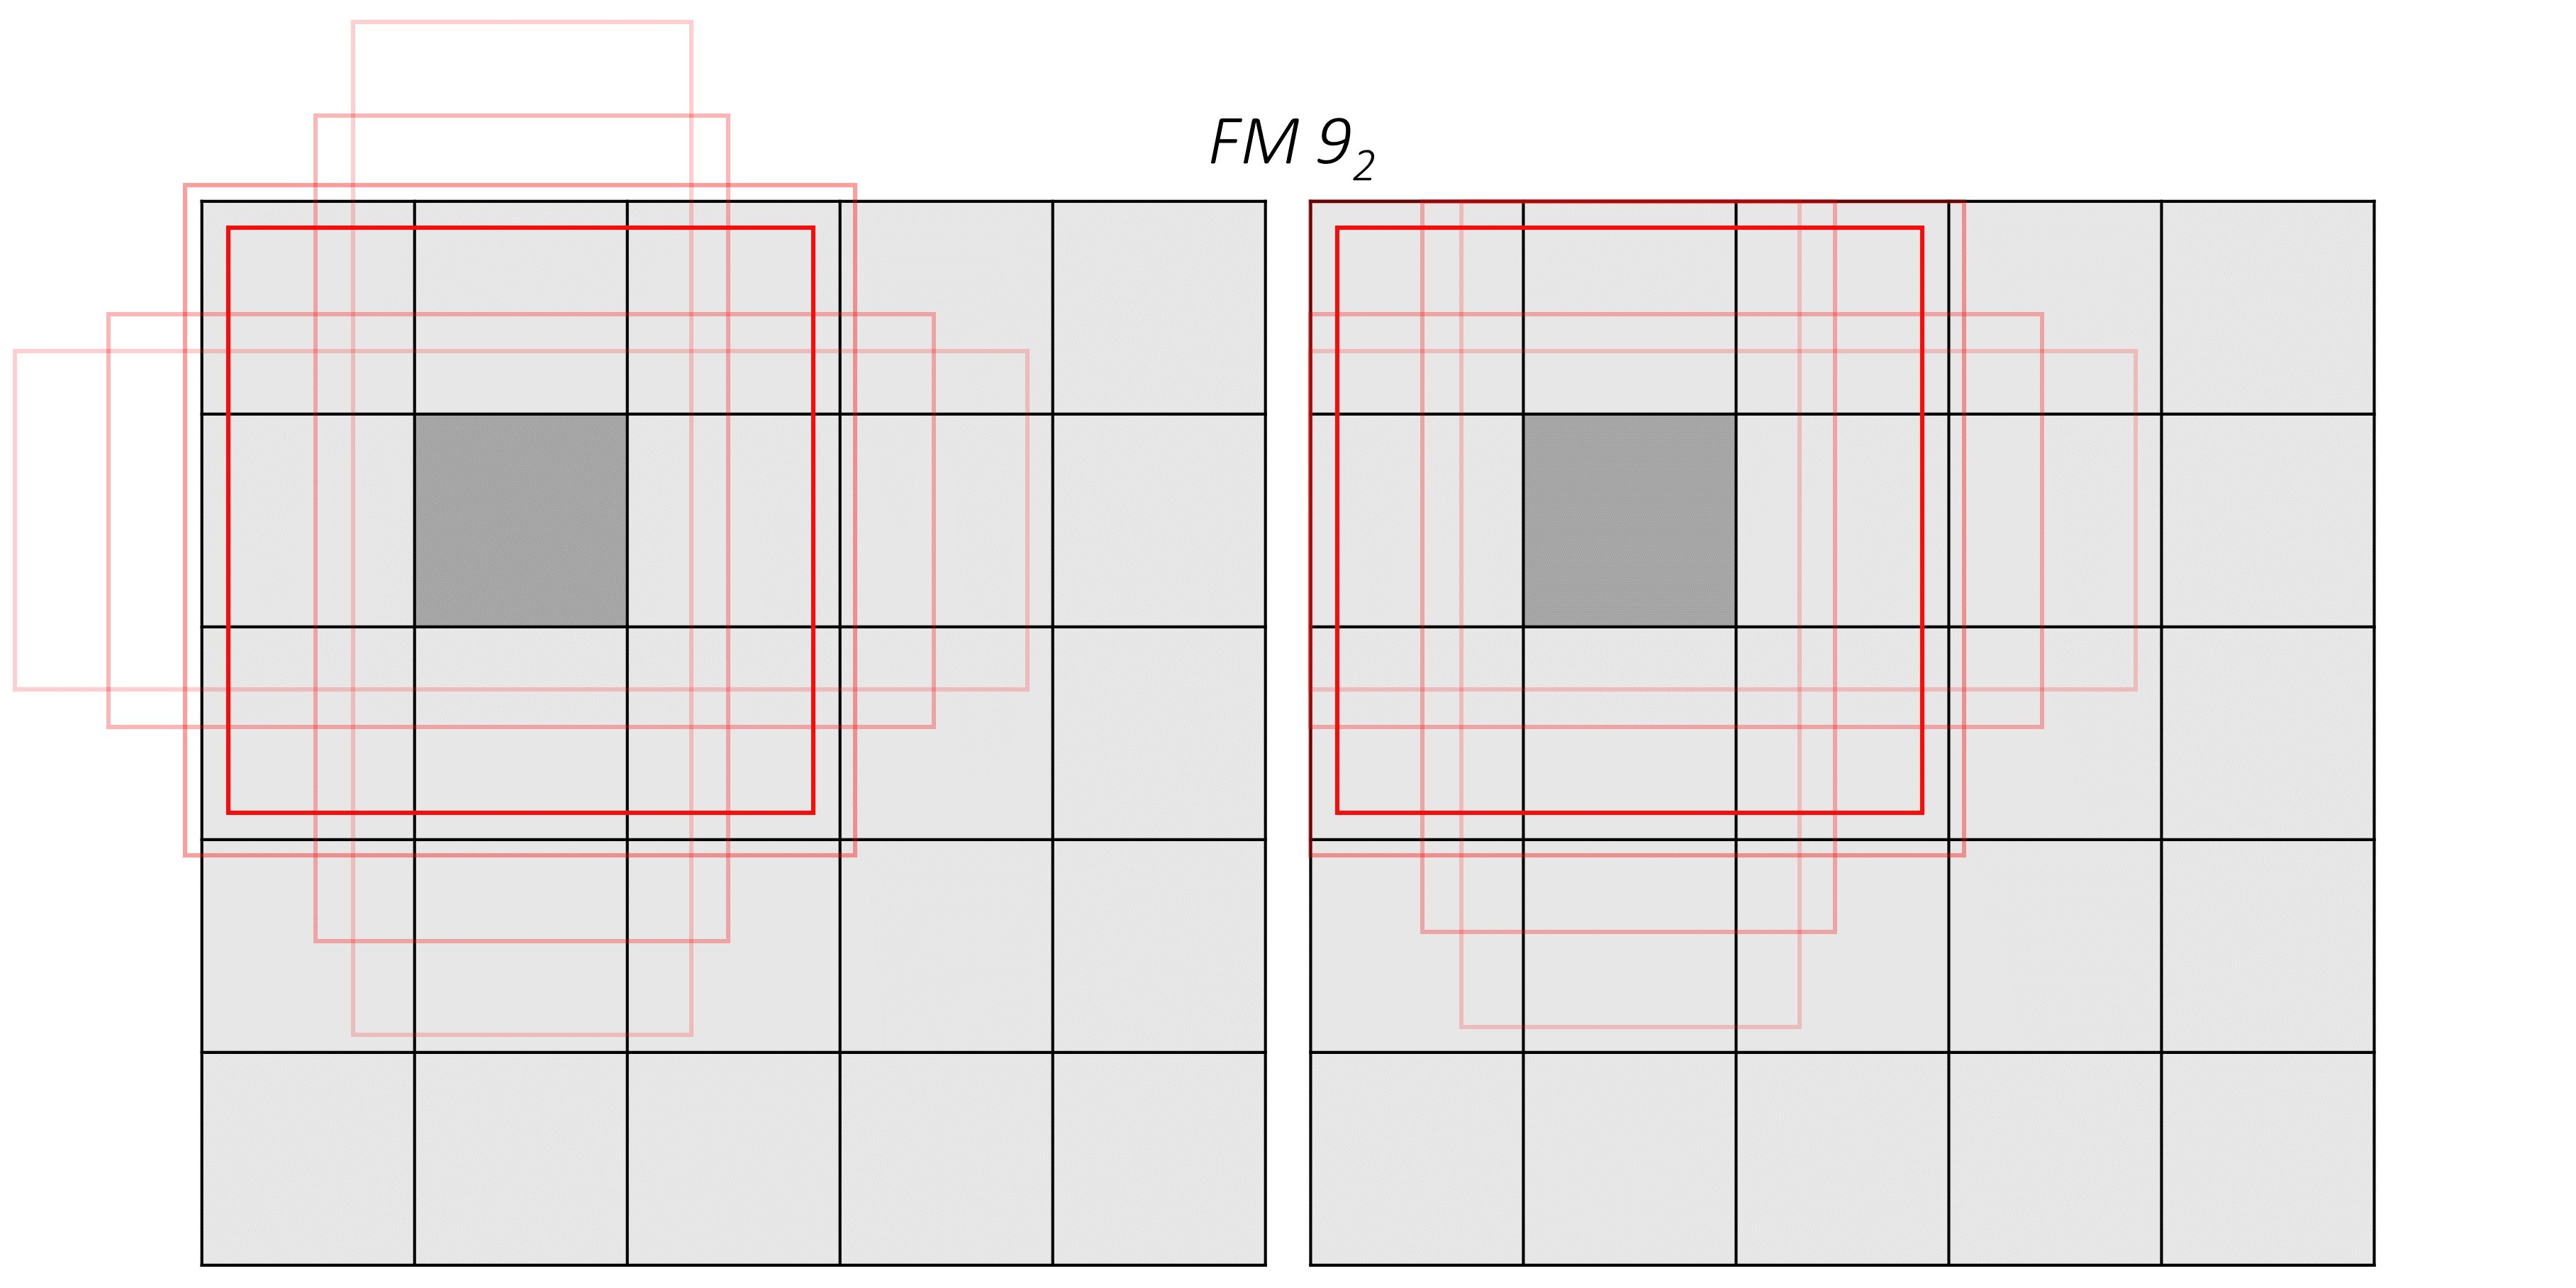
\includegraphics[width=\linewidth]{fig/priors2.jpg}
  \caption{Prior boxes for feature map 9\_2. When priors at a location overshoot the edges of the feature map, they are clipped.}\label{fig:prior}
\end{figure}

\subsection{Prediction convolutions}
We use each prior as an approximate starting point and then find out how much it needs to be adjusted to obtain a more exact prediction for a bounding box. So we need to predict the offset of the box to the priors. Besides, we also need $n$ scores for each bounding box to show its confidence in each class.

To do this in the simples manner, we use two convolutional layers for each feature map:
\begin{itemize}
  \item a localization prediction convolutional layer with a $3\times 3$ kernel evaluating at each location (i.e. with padding and stride of 1) with 4 filters for each prior present at the location, which calculate the four encoded offsets $(g_{c_x}, g_{c_y}, g_w, g_h)$ for the bounding box predicted from that prior.

  \item a class prediction convolutional layer with a $3\times 3$ kernel evaluating at each location  with $n$ filters for each prior present at the location
\end{itemize}

\subsection{Non-Maximum Suppression}
Following the above procedures, we have $8732$ candidate boxes. To eliminate the inaccurate ones, we need to use what is called Non-maximum suppression (NMS). Algorithmically, it is carried out as follows:

Upon selecting candidates for each non-background class,
\begin{enumerate}
  \item Arrange candidates for this class in order of decreasing likelihood.

  \item Consider the candidate with the highest score. Eliminate all candidates with lesser scores that have a overlap of more than, say, 0.5 with this candidate.

  \item Consider the next highest-scoring candidate still remaining in the pool. Eliminate all candidates with lesser scores that have a overlap of more than 0.5 with this candidate.

  \item Repeat until you run through the entire sequence of candidates.
\end{enumerate}

% The end result is that you will have just a single box – the very best one – for each object in the image.






\section{SSD Improvement}
\subsection{Basics}
To facilitate our later three improvements, we need to first slightly change the network structure. First, we enlarge the network by applying the SSD512 configuration, which
\begin{enumerate}
  \item Increase input size to $512\times 512$
  \item Add two more convolutional layers for auxiliary convolutions, which increases the number of feature maps from $6$ to $7$.
\end{enumerate}

Then, for feature map fusion discussed below, we need only five feature maps, so we remove two convolutional blocks, one from vgg and one from extra layers.

To implement the changes in the code, we modify the configuration variables in \code{ssd.py} and \code{data/config.py}. To make our new code compatible with original SSD300, we add a few parameters to specify which model to use in the training/evaluate process.

Specifically, in the top function \code{build\_ssd}, we add a parameter \code{extension}, which is a list of options that we can add to the network. Our later improvement is carried out in this framework to ensure compatibility. The structure of our improvement basics is shown in Figure~\ref{fig:basics}

\begin{figure*}[htbp]
  \centering
  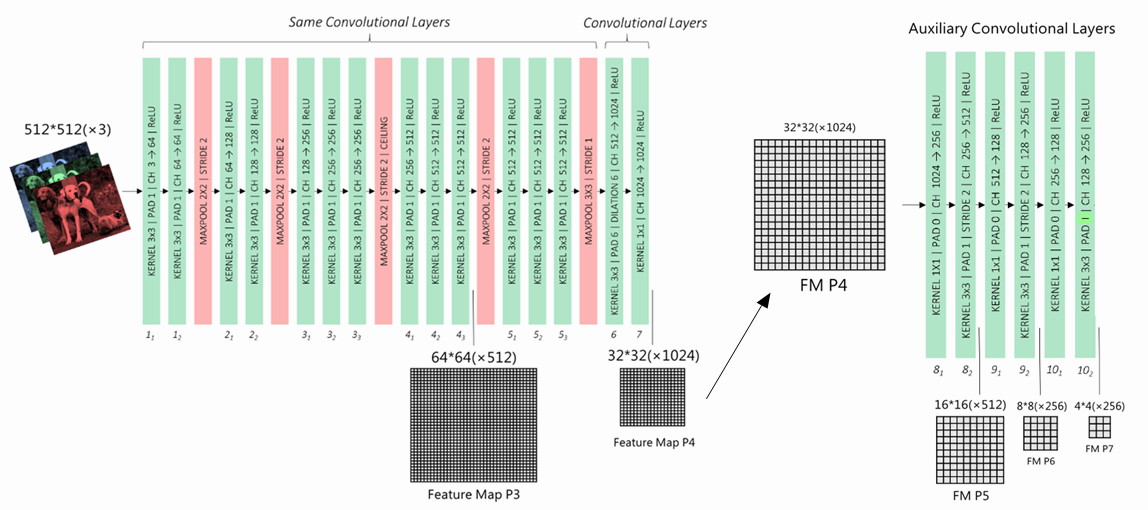
\includegraphics[width=\linewidth]{fig/basics.png}
  \caption{Backbone structure for our improvement}\label{fig:basics}
\end{figure*}

% ljy
\subsection{Super Resolution}
Original images in the VOC dataset are around $300$ in size. To feed them to the $512$ input, we can naively use interpolation to resize the images, but that will make them vague and lose some details. So we use Enhanced Deep Residual Networks (EDSR) for image super-resolution \cite{edsr}. It can enlarge the images while retaining some details, as shown in Figure~\ref{fig:edsr}. We use EDSR to double the size of original images, then use downsampling methods to resize them to fit the $512$ input size.

\begin{figure}[htbp]
  \centering
  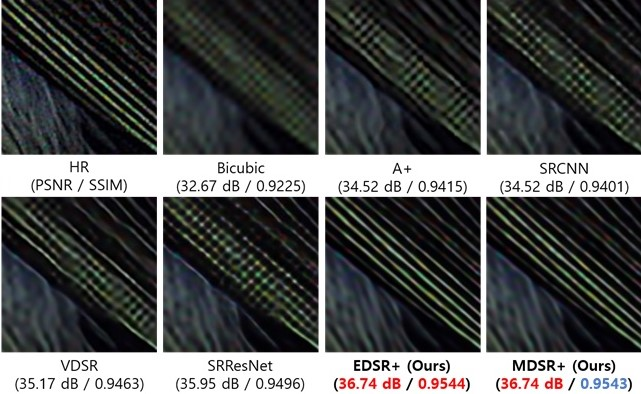
\includegraphics[width=\linewidth]{fig/edsr.png}
  \caption{Performance of EDSR compared with other methods. HR is the true high resolution image.}\label{fig:edsr}
\end{figure}

% chp
\subsection{Feature Fusion}
We use BiFPN as our method of feature fusion, which is inspired by EfficientDet \cite{EfficientDet} proposed by Google research group one month ago. In the original paper, the backbone network is EfficientNet, which is a light-weighted network with less parameters published by Google in May, 2019. The backbone network serves only as feature extractor, which generates feature maps with different resolutions, we use vgg16 instead to easily accommodate with our SSD detection. As mentioned above, we use a $512\times 512$ image (obtained from image super-resolution) as input and pass it through vgg-16 to get five feature maps $P_3,P_4,\ldots,P_7$ in sequence, where $P_3$ represents the feature map of size $64\times 64$, and $P_7$ represents the feature map with size $4\times 4$.

The convolutional FPN aggregates multi-scale features in a top-down manner:
\begin{align*}
  P_7^{out} & =Conv(P_7^{in})                   \\
  P_6^{out} & =Conv(P_6^{in}+Resize(P_7^{out})) \\
  \ldots    &                                   \\
  P_3^{out} & =Conv(P_3^{in}+Resize(P_4^{out})) \\
\end{align*}

where Resize is usually an up-sampling or down-sampling op for resolution matching, and Conv is usually a convolutional op for feature processing.

To address the issue of one-way flow information limitation, our BiFPN layer adds an extra bottom-up path aggregation network, which idea is inspired by PANet. The idea of PANet is shown in Figure~ref{fig:bifpn}.

\begin{figure}[htbp]
  \centering
  \subfigure[PANet]{
    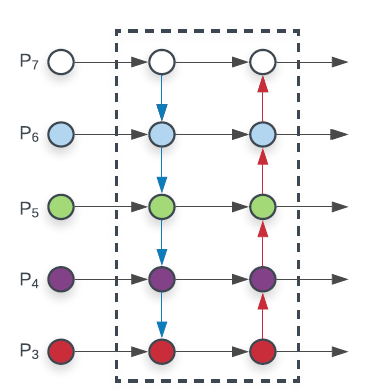
\includegraphics[width=0.45\linewidth]{fig/panet.png}
  }
  \subfigure[BiFPN]{
    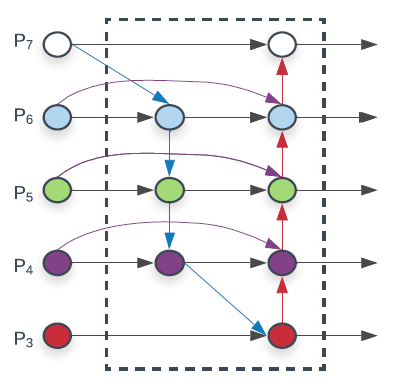
\includegraphics[width=0.45\linewidth]{fig/bifpn.png}
  }
  \caption{From PANet to BiFPN}\label{fig:bifpn}
\end{figure}

However, for better feature fusion and increased efficiency, BiFPN has made the following improvements:

\subsubsection{Cross-scale connections}
\begin{itemize}
  \item We remove those nodes that only have one input edge.
        This is because: if a node has only one input edge with no feature fusion, then it will have less contribution to feature network that aims at fusing different features.
  \item Add and extra edge from the original input to output node. This is for further feature fusion without adding much cost
  \item We treat the BiFPN layer as one feature layer, and repeat the same layer multiple times to enable more high-level feature fusion. (In EfficientDet-d0 in our work, we repeat the BiFPN network twice in sequence.
\end{itemize}

\subsubsection{Weighted feature fusion}
For different layers of input features may have different contribution the final prediction in each level of the output feature map. We introduce a weighted feature fusion as a kind of self-attention mechanism. That is, we add linear weights for input feature maps to obtain the intermediate feature map, and we also add linear weights for intermediate feature maps to obtain output feature for a BiFPN layer. The final formulas of obtaining features of different levels in the feature map in a BiFPN layer is defined as follows:

\begin{figure*}[htbp]
  \centering
  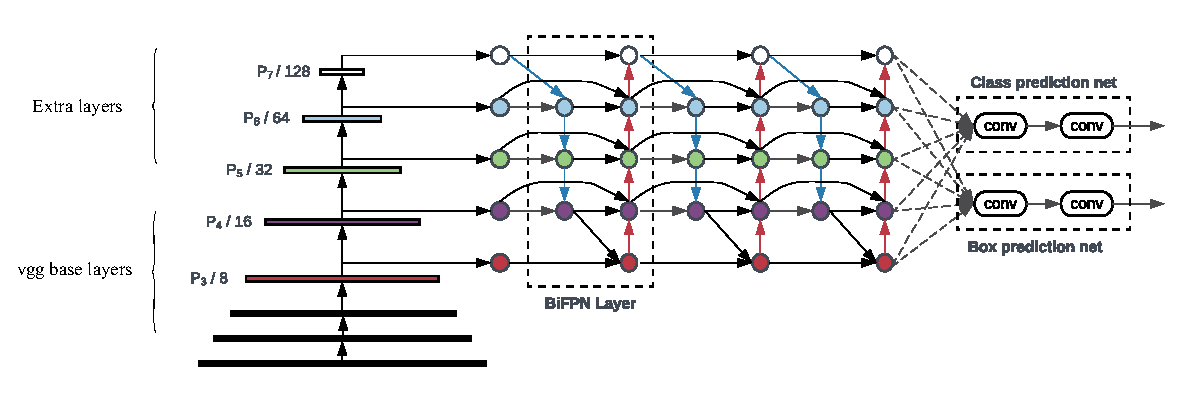
\includegraphics[width=\linewidth]{fig/ssd_bifpn.eps}
  \caption{Architecture of our SSD-BiFPN network}\label{fig:arch}
\end{figure*}

\begin{figure*}[htbp]
  \centering
  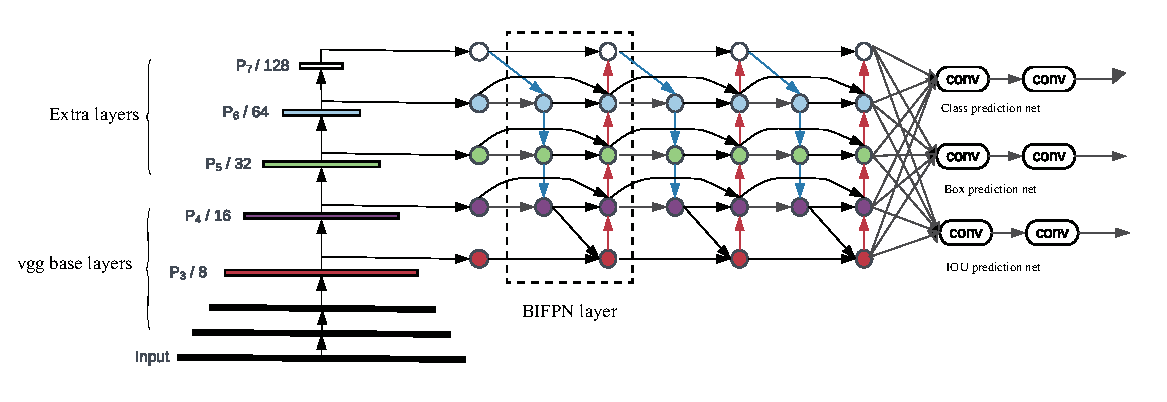
\includegraphics[width=\linewidth]{fig/ssd_iou.eps}
  \caption{Architecture of our SSD-BiFPN-IoU network}\label{fig:iou}
\end{figure*}

\begin{align*}
  P_6^{td}  & =Conv\left(\frac{w_1\cdot P_6^{in}+w_2\cdot Resize(P_7^{in})}{w_1+w_2+\epsilon}\right)                              \\
  P_6^{out} & =Conv\left(\frac{w_1'\cdot P_6^{in}+w_2'\cdot P_6^{td}+w_3'\cdot Resize(P_5^{out})}{w_1'+w_2'+w_3'+\epsilon}\right)
\end{align*}
where $P_6^{td}$ is the intermediate feature at level 6 on the top-down pathway, and Pout6 is the output feature at level 6 on the bottom-up pathway. All other features are constructed in a similar manner.

\subsubsection{Architecture}
The final structure of the whole network including the vgg-16 backbone, BiFPN layers, and the prediction head is shown in Figure~\ref{fig:arch}:


% chp
\subsection{IOU Loss}
The low correlation between the classification score and localization accuracy of the predicted detections has severely hurt the localization accuracy of models. To solve this problem, IoU-aware single-stage object detector is proposed. Specifically, IoU-aware single-stage object detector predicts the IoU between the regressed box and the ground truth box. Then the classification score and predicted IoU are multiplied to compute the detection confidence, which is highly correlated with the localization accuracy. The detection confidence is then used as the input of NMS and VOC AP computation, which will substantially improve the localization accuracy of models.

\subsubsection{Model architecture}
We design a IoU prediction head parallel with the regression head and the classification head to predict the IoU between each regressed anchor and the ground truth box. The modified architecture with BiFPN layer is shown in Figure~\ref{fig:iou}:

To keep the model's efficiency, the IoU prediction head consists of only assign $3\times 3$ convolution layer, followed by a sigmoid activation layer, ensuring the predicted IoU is in the range of $[0, 1]$.

\subsubsection{Loss function}
The loss of IoU of a sample is the cross entropy between predicted IOU and truth IoU of regressed prior box and its assigned ground truth box. We only consider IoU loss of positive samples where truth IoU is greater than the threshold. The loss function formula is described in training part, with other classification loss and confidence loss.


\section{Experiments}
% \begin{figure*}[htbp]
%   \centering
%   \subfigure[Extra Small]{
%     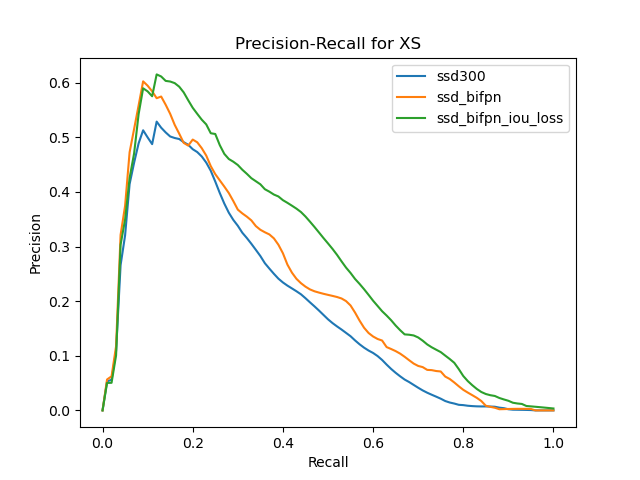
\includegraphics[width=0.45\linewidth]{fig/XS_pr.png}
%   }
%   \subfigure[Small]{
%     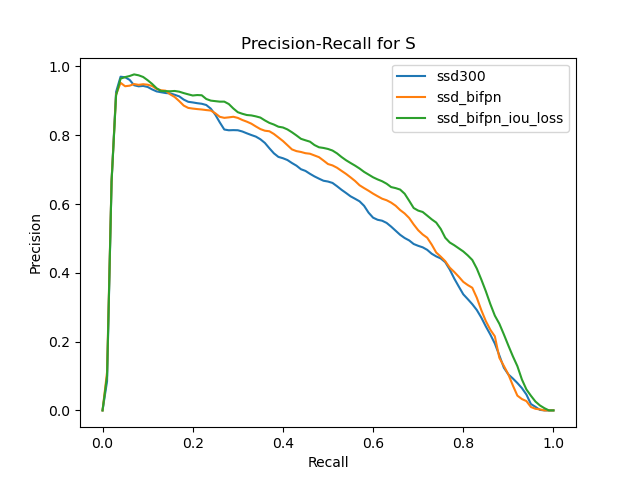
\includegraphics[width=0.45\linewidth]{fig/S_pr.png}
%   }
%   \caption{Precision-Recall graph}\label{fig:res}
% \end{figure*}

% ljy
\subsection{Dataset}
We use the Pascal VOC data sets \cite{voc} for our training and evaluation. Specifically, VOC2007 constains 20 classes:
\begin{itemize}
  \item Person: person
  \item Animal: bird, cat, cow, dog, horse, sheep
  \item Vehicle: aeroplane, bicycle, boat, bus, car, motorbike, train
  \item Indoor: bottle, chair, dining table, potted plant, sofa, tv/monitor
\end{itemize}

It has a split of Train/validation/test, which contains $9963$ images with $24640$ annotated objects. We augment the dataset by using EDSR, so that there is a original type and super-resolution type for each image.

% chp
\subsection{Training}
We evaluate our four models of \code{ssd300}, \code{ssd\_bifpn}, and \code{ssd\_bifpn\_iou\_loss} on the VOC2007 detection datasets, and an additional option whether to use super-resolution input pictures. The setting of parameter is quite similar to the settings in the original paper. Each model is trained using SGD optimizer with momentum $0.9$ and weight decay $4\times 10^{-5}$.  Learning rate is initially $0.001$ and then annealed down using cosine decay rule. Batch normalization is added after every convolution with batch norm decay $0.997$ and epsilon $10^{-4}$. We use exponential moving average with decay $0.9998$. We also employ commonly-used focal loss with $\alpha = 0.25$ and $\gamma= 1.5$, and aspect ratio $\{1/2, 1, 2\}$. Our models are trained with batch size $16$ on RTX 2080 Ti chips.

As the same to RetinaNet, focal loss is adopted for the classification loss and the smooth $L_1$ loss is adopted for the regression loss as Equ~\eqref{eq1} and \eqref{eq2} show.

\begin{align}
  L_{cls} & =\frac{1}{N_{pos}}\left(\sum_{i\in pos}^N FL(p_i,\hat{p}_i)+\sum_{i\in neg}^M FL(p_i,\hat{p}_i)\right)\label{eq1} \\
  L_{loc} & =\frac{1}{N_{pos}}\sum_{i\in pos}^N \sum_{m\in \{cx,cy,w,h\}} \text{smooth}_{L_1}(l_i^m-\hat{g}_i^m)\label{eq2}
\end{align}

Because the predicted IoU is in the range of $[0,1]$, binary cross-entropy loss is adopted for the IoU prediction loss as Equ~\eqref{eq3} shows.

\begin{equation}
  L_{IoU}=\frac{1}{N_{pos}}\sum_{i\in pos}^N CE(IoU_i,\hat{IoU}_i)\label{eq3}
\end{equation}

During training, the IoU prediction head is trained jointly with the classification head and regression head. In model \code{ssd300} and \code{ssd\_bifpn}, the total loss is the sum of classification loss and regression loss, which is the same as SSD, while in model \code{ssd\_bifpn\_iou\_loss}, the total loss is calculated as the sum of classification loss, regression loss and iou loss, which is shown in Equ~\eqref{eq4}.

\begin{equation}
  L_{total}=L_{cls}+L_{loc}+L_{IoU}\label{eq4}
\end{equation}

% ljy
\subsection{Evaluation}
In order to evaluate the performance on different scales of detections, we first divide all the ground-truth objects depending on the object’s percentile size within its category, i.e. EACH OBJECT CATEGORY has its OWN split of scales:
\begin{itemize}
  \item extra-small (XS: bottom 10\%)
  \item small (S: next 20\%)
  \item medium (M: next 40\%)
  \item large (L: next 20\%)
  \item extra-large (XL: next 10\%)
\end{itemize}

We write \code{voc\_mark\_size.py} to label each ground-truth detections and save them to pickle files for reference.

For the evaluation metrics, we use recall, precision and AP. We modify \code{eval.py} so that each metric for each scale of each category is calculated and stored. As a basics for these three metrics, we need to adapt the true positive (TP) and false positive (FP) to different scales. Formula for TP is obvious, one detection's scale corresponds to the scale of its ground-truth. For FP, the mismatched detection falls into the scale of the scale of its own, because it is not matched to any ground-truth.

\subsection{Results}
The performance of our model in VOC2007 test is shown in Table~\ref{tab:res} and Figure~\ref{fig:res}. We can see that our models outperform the baseline in both XS and S objects while the performance on all scales also has a slight improvement.

\begin{table}[htbp]
  \centering
  \caption{PASCAL VOC2007 test results}\label{tab:res}
  \begin{tabular}{|l|c|c|c|c|c|c|}
    \hline
     & \multicolumn{3}{|c|}{mAP}    \\
    \hline
                  & XS     & S      & Total \\
    \hline
    SSD300        & 0.2808 & 0.6079 & 0.7770 \\
    SSD+BiFPN     & 0.3407 & 0.6319 & 0.7667  \\
    SSD+BiFPN+IoU & \textbf{0.3732} & \textbf{0.6711} & \textbf{0.7957}\\
    \hline
  \end{tabular}
\end{table}

\begin{figure}[htbp]
  \centering
  \subfigure[Extra Small]{
    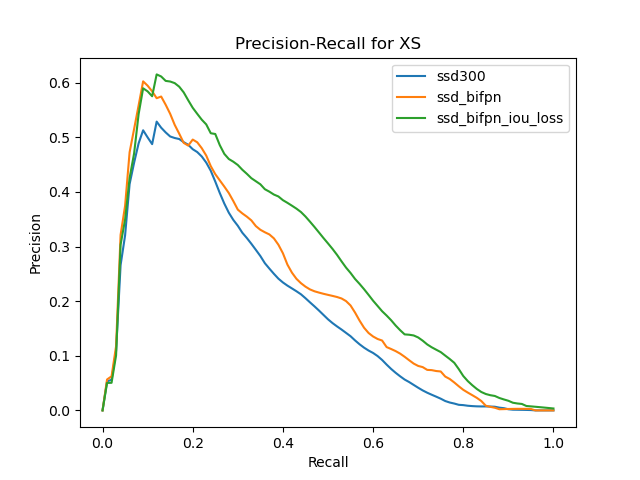
\includegraphics[width=0.9\linewidth]{fig/XS_pr.png}
  }
  \subfigure[Small]{
    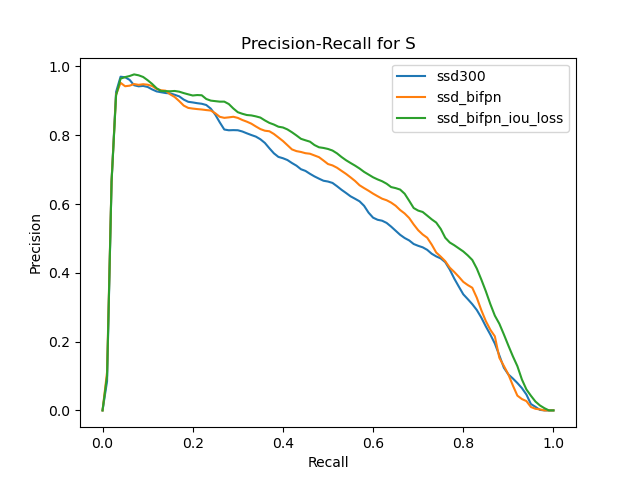
\includegraphics[width=0.9\linewidth]{fig/S_pr.png}
  }
  \caption{Precision-Recall graph}\label{fig:res}
\end{figure}

\section{Conclusion}


\bibliographystyle{IEEEtran}
\bibliography{Ref}


% that's all folks
\end{document}